% !TeX root =../../main.tex

\chapter{Introduction} \label{ch:introduction}


\section{Motivations and Challenges}
Software systems usually suffer from various kinds of vulnerabilities and weakness. These vulnerabilities can cause huge catastrophes from financial property loss to massive personnel casualty. For example, \emph{Heartbleed}~\cite{heartbleed}(CVE-2014-0160) is a critical vulnerability caused by an implementation defect in the widely used OpenSSL cryptographic software library which can compromise the integrity of communications across the entire Web. Further, it is reported that this may also affect the internal networks of enterprise in the coming years due to the fact that most enterprises do not have a good handle on the SSL encrypted services. It is also interesting that this vulnerability was introduced in 2012 while was not discovered until 2 years later in 2014. Worse still, it also remains unknown when all the mainstream services will be upgraded to get grid of this vulnerability eventually. Other software weakness may lead to more direct tragedies which lead to deaths. For example, the aircraft accident of Ethiopian Airlines Flight 302 in the late 2018 is high likely due to the improper functionality of the Maneuvering Characteristics Augmentation System (MCAS) from Boeing 737 Max~\cite{boeing_Ethiopian}. 153 lives were lost during this accident, including 149 passengers and 8 crew. Ironically, MCAS is designed to keep the balance of the airplane. The same Boeing 737 Max jet led to totally 189 people's death during Lion Air Flight 610 in 2019, which probably results from the functionality of MCAS.

\section{Main Work}

\section{Contributions of the Thesis}

\begin{figure}[ht]
	\begin{center}
		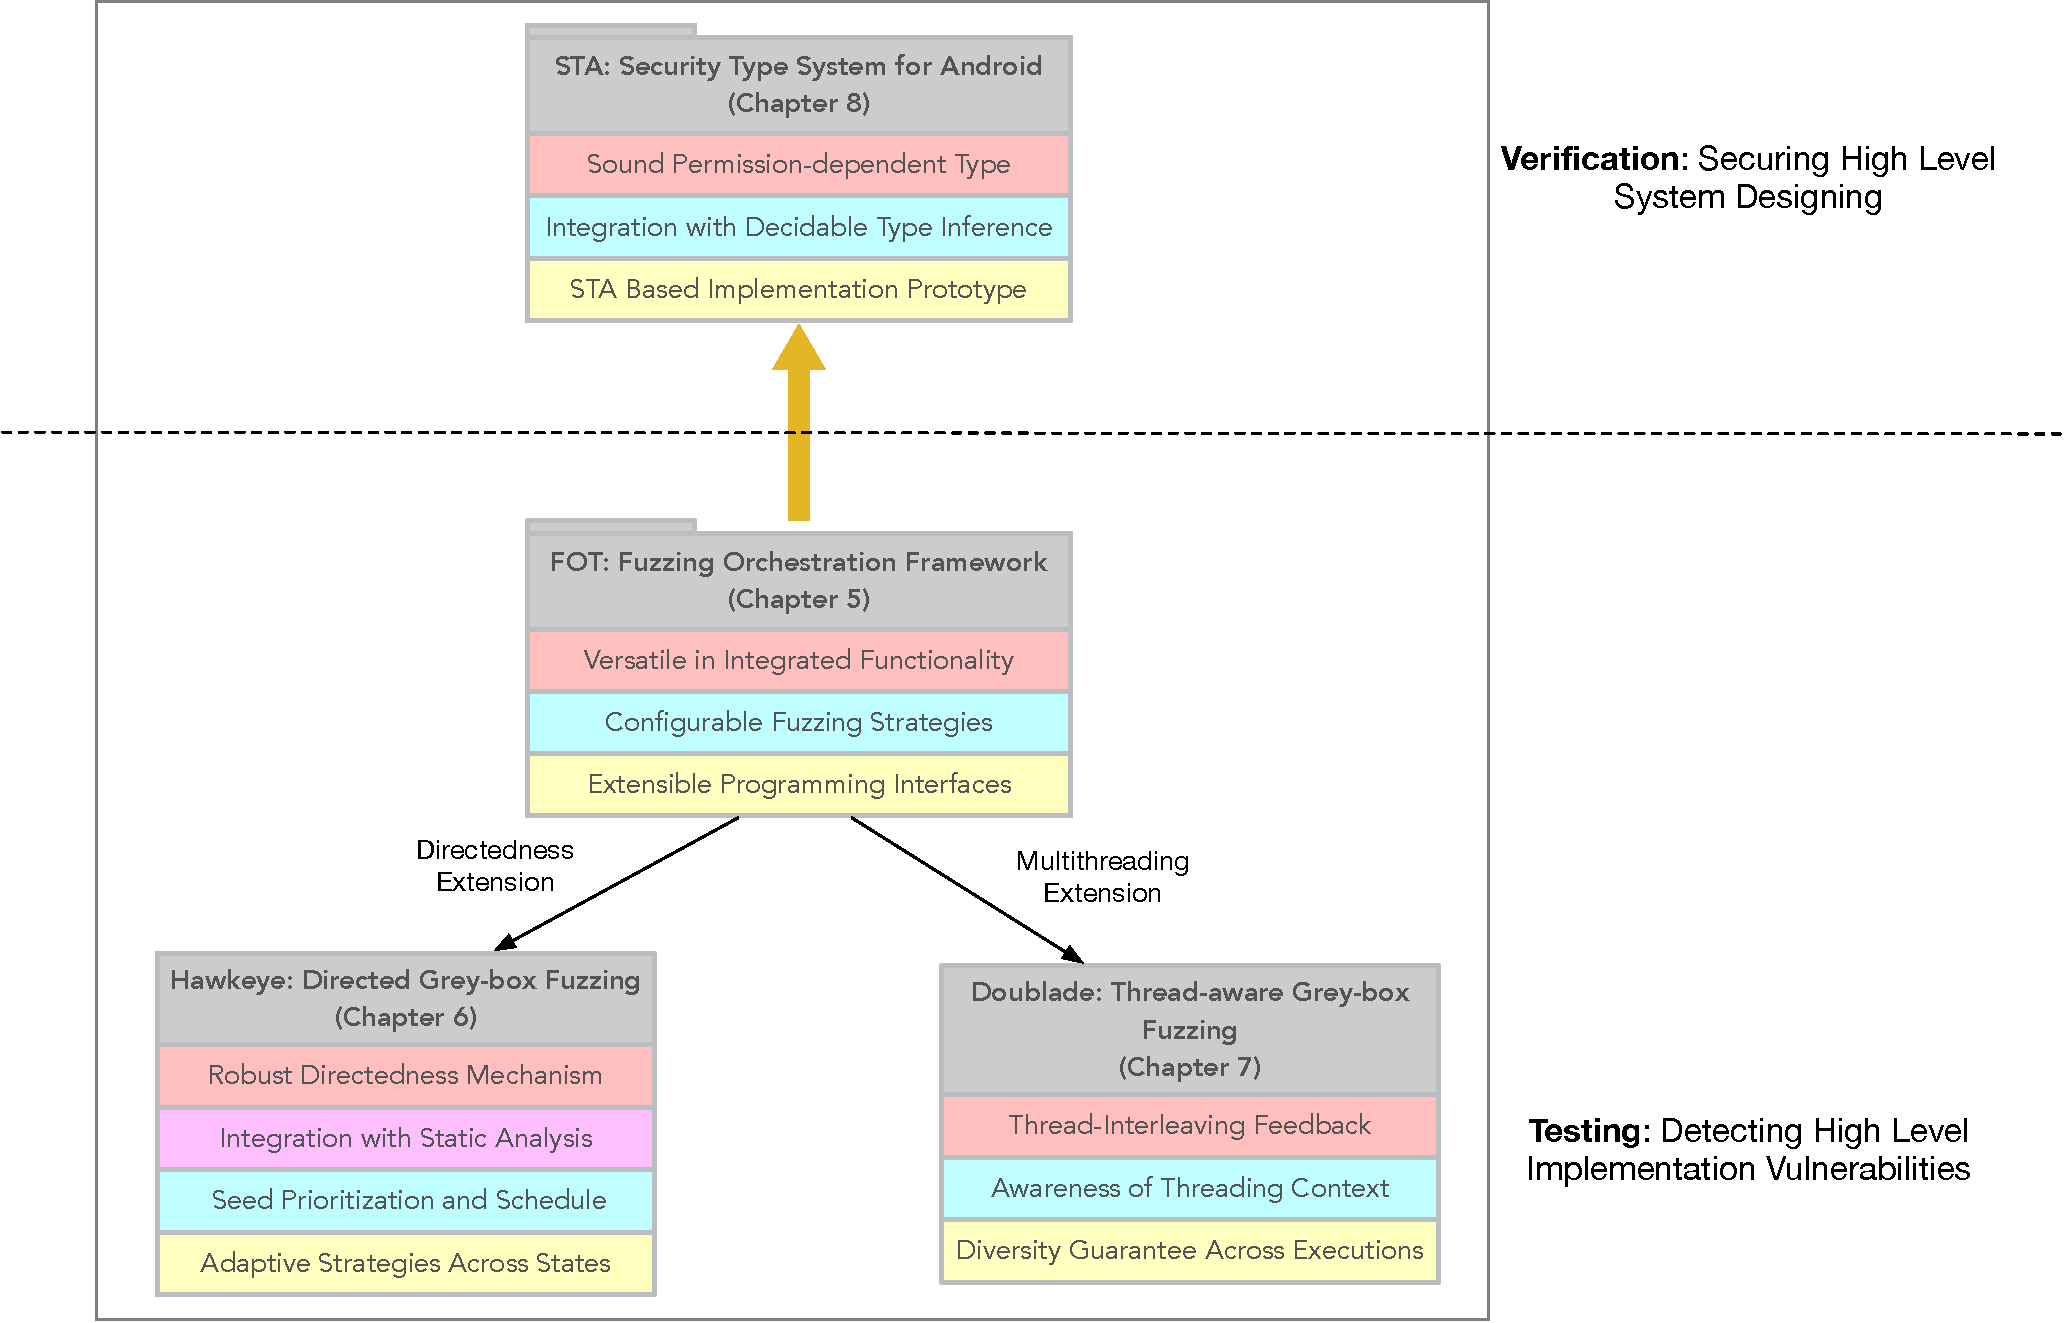
\includegraphics[width=0.98\textwidth]{res/contributions}
		\caption{Contributions of the Thesis and their Relations}
		\label{fig:works}
	\end{center}
\end{figure}


\section{List of Materials Related to the Thesis}
\begin{enumerate}
	\item \myname, Yuekang Li, Bihuan Chen, Yinxing Xue, Yang Liu, ``FOT: A Versatile, Configurable, Extensible Fuzzing Framework'', ESEC/FSE 2018 Proceedings of the 2018 26th ACM Joint Meeting on European Software Engineering Conference and Symposium on the Foundations of Software Engineering, Pages 867-870, \url{http://doi.acm.org/10.1145/3236024.3264593}, DOI: 10.1145/3236024.3264593.
	\item \myname, Yinxing Xue, Yuekang Li, Bihuan Chen, Xiaofei Xie, Xiuheng Wu, Yang Liu, ``Hawkeye: Towards a Desired Directed Grey-box Fuzzer'', CCS '18 Proceedings of the 2018 ACM SIGSAC Conference on Computer and Communications Security, Pages 2095-2108, \url{http://doi.acm.org/10.1145/3243734.3243849}, DOI: 10.1145/3243734.3243849.
	\item \myname, Shengjian Guo, Yinxing Xue, Yulei Sui, Cen Zhang, Yuekang Li, Haijun Wang, Yang Liu, ``Doublade: Enhancing Grey-box Fuzzing for Multithreaded Programs with Thread-aware Analysis'', ESEC/FSE 2019, The 27th ACM Joint European Software Engineering Conference and Symposium on the Foundations of Software Engineering.
	\item \myname, Alwen Tiu, Zhiwu Xu, Yang Liu, ``A Permission-Dependent Type System for Secure Information Flow Analysis'', 2018 IEEE 31st Computer Security Foundations Symposium (CSF), Oxford, 2018, pp. 218-232. \url{https://doi.org/10.1109/CSF.2018.00023}, DOI: 10.1109/CSF.2018.00023. A technical report is available at \url{https://arxiv.org/abs/1709.09623}.
\end{enumerate}

\section{Outline of the Thesis}

The rest of this thesis is organized as follows.

Chapter~\ref{ch:fot} describes the recent progress of fuzzing and several aspects of challenges, and introduces our grey-box fuzzing framework, \FOT, which aims to solve these issues. Chapter~\ref{ch:dfot} explains our directed grey-box fuzzer \dFOT built on top of \FOT; \dFOT is our attempt to guide the fuzzing process to specific program targets. Chapter~\ref{ch:mtfuzz} describes \mtfuzz based on \FOT, which aims to enhance the effectiveness of fuzzing on multithreaded programs. Chapter~\ref{ch:sta} describes our attempt to secure software systems based on verification, which applies a permission-dependent type system to enforce the non-interference property that prevents the information leakage in an Android-like system. Chapter~\ref{ch:discuss} discusses my reflection on the testing and verification based techniques. Chapter~\ref{ch:conclusion} concludes this thesis and describes the possible future work.